\section{Introduction}
\label{sec:introduction}

GPU performance engineering is still fundamentally measurement-driven.
Developers usually optimize kernels by compiling candidate variants, running them on the target accelerator, profiling hardware counters, and then deciding whether to focus on computation, memory traffic, or both.
That workflow is already costly for humans, and it becomes even more expensive in agentic software-engineering loops where an LLM proposes many candidate edits and expects profiler feedback after each one \cite{liRiseAITeammates2025,gongLanguageModelsCode2025,ouyangKernelBenchCanLLMs2025,chenCUDALLMLLMsCan2025,zhangCudaForgeAgentFramework2025,kaplanParaCodexProfilingGuidedAutonomous2026}.

\begin{figure}[t]
  \centering
  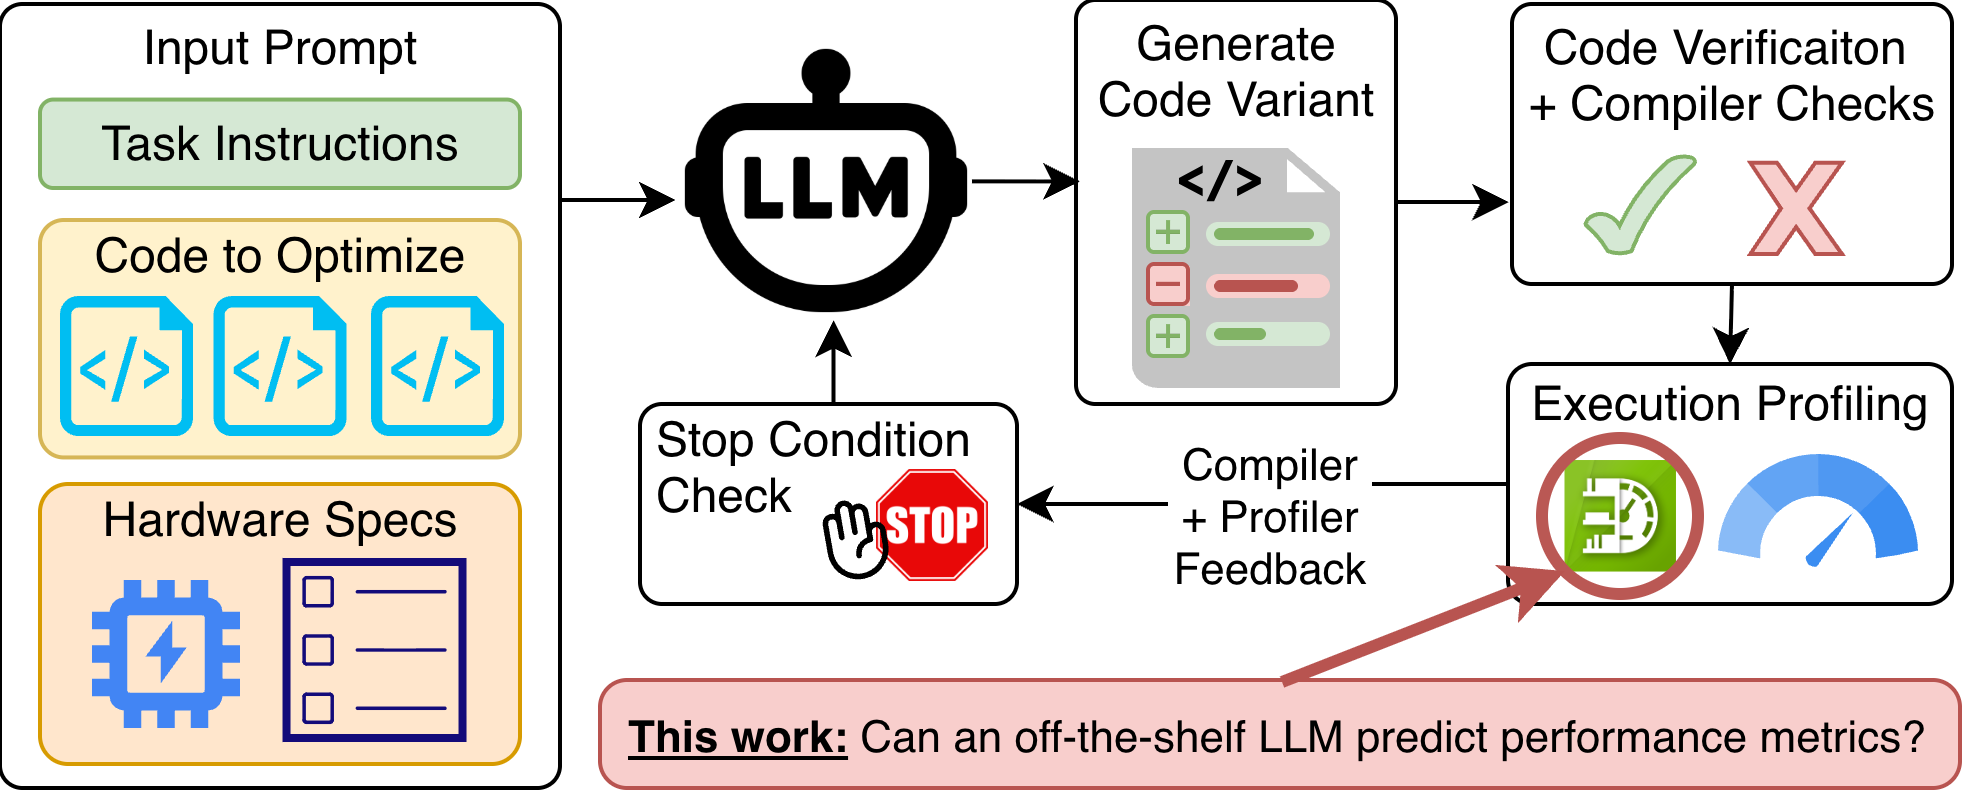
\includegraphics[width=\linewidth]{figures/optimization_loop.png}
  \caption{Profiler-in-the-loop GPU optimization is effective, but it assumes repeated access to the target accelerator.
  This paper studies whether LLMs can provide an execution-free triage signal earlier in that loop, before runtime profiling is available.}
  \Description{A diagram contrasting the usual compile-run-profile optimization loop with an earlier execution-free triage step that reasons from software artifacts before scarce GPU profiling time is used.}
  \label{fig:optimization-loop}
\end{figure}

In practice, target-GPU access is often the bottleneck.
Accelerators may be rationed on a shared cluster, unavailable in early development, blocked by missing system dependencies, or simply too expensive to occupy for speculative triage.
The problem is therefore not ``can LLMs replace profilers?''; it is whether they can provide a smaller, earlier, and still interpretable signal that helps developers and tools decide where scarce profiling effort should be spent first.

We focus on one such signal: Roofline Arithmetic Intensity (\rai), the ratio of floating-point work to DRAM traffic in the Roofline model \cite{samuelwilliamsRooflineInsightfulVisual2009}.
\rai is attractive for software engineering because it is both profiler-relevant and interpretable.
It does not directly predict runtime, but it does give a developer or tool builder an early indication of whether a kernel is likely to sit on the memory side or the compute side of a target GPU's Roofline balance point.
That makes it a plausible triage target for LLM-based development tools that must reason from software artifacts before execution.

This paper studies whether off-the-shelf LLMs can estimate profiler-derived \rai from source code, build context, command-line inputs, and optional post-compilation artifacts such as SASS.
Our setting is execution-free at prediction time: the models do not execute or profile the target kernel when producing a prediction.
Ground truth, however, is profiler-derived and comes from an offline benchmark-building process.
We therefore ask a deliberately narrower question than general performance prediction:
\textit{Can off-the-shelf LLMs provide an execution-free early triage signal for GPU kernels by estimating DRAM-level \rai from software artifacts?}

To answer that question, we build on 95 HeCBench CUDA and OpenMP programs.
They expose 254 first-invocation GPU kernels and 1{,}016 kernel-device rows across an RTX~3080, A10, A100, and H100.
We compare \sourceonly prompts against \sourcesass prompts for three off-the-shelf models: \gptfivefour, \opus, and \gptoss.
The released evaluation subset contains 5{,}766 completed model queries, which yield 17{,}298 precision-specific FP16/FP32/FP64 \rai predictions.
This lets us study not only numerical \rai error, but also zero-versus-nonzero detection, nonzero bandwidth-bound versus compute-bound triage, prompt-evidence effects, cost/latency tradeoffs, and recurring failure patterns.

Three findings matter most.
First, source-only reasoning is often good enough for nonzero FP32/FP64 triage, but it collapses for FP16.
Second, SASS helps substantially when compiler-realized behavior matters, especially for FP16 and for frontier-model triage decisions.
On the 732 kernel-device rows shared across all paper configurations, \sourcesass improves nonzero FP16 balanced triage accuracy from the trivial 0.50 baseline to 0.870 for \gptfivefour and 0.984 for \opus.
Third, the signal is strong enough to prioritize scarce profiling effort:
at a 10\% profiling budget, \sourcesass \gptfivefour and \opus recover all shared-subset FP16 compute-bound rows, while source-only FP32 rankings already recover 82\% and 96\% of the true compute-bound rows.
The benchmark is also not ``LLMs versus nothing'':
context-only, deterministic, and lightweight learned static baselines recover substantial triage signal and even exceed one-shot prompting in a few source-only FP16 and \sourcesass FP64 settings, but they remain poor numeric \rai regressors and still trail the frontier models on \sourcesass FP16/FP32 triage.
The cheapest model is still a useful low-cost source-only point, but it is less complete and makes far weaker use of SASS than the frontier models.

The paper's contribution is therefore squarely about software engineering.
We study how execution-relevant software artifacts can support AI-assisted performance reasoning before execution.
We package that task as a benchmark and empirical study, show where off-the-shelf prompting is already useful, and identify where it remains unreliable.

More concretely, this paper makes four contributions:
\begin{itemize}[leftmargin=1.2em]
  \item We formulate execution-free \rai prediction as a software-engineering task for early GPU-kernel triage.
  Inputs are software artifacts, and ground truth is profiler-derived DRAM-level \rai.
  \item We report an empirical study across 254 CUDA/OpenMP kernels and four NVIDIA GPUs, with explicit task splits for zero/nonzero detection, nonzero \rai regression, nonzero \bandwidthbound/\computebound triage, and fixed-budget compute-bound retrieval.
  \item We quantify the effect of post-compilation artifacts against context-only, deterministic, and lightweight learned static baselines.
  SASS materially helps the frontier models, but different static methods win in different regimes.
  \item We package the benchmark, prompts, responses, and plotting artifacts for follow-on work, while documenting the method's limits so future work can compare against stronger static baselines and better-validated failure analyses.
\end{itemize}

The remainder of the paper is organized as follows.
Section~\ref{sec:related-work} positions the paper relative to Roofline analysis, execution-free GPU performance prediction, and LLM-based optimization.
Sections~\ref{sec:task-methodology} and \ref{sec:study-design} define the prediction task and study design.
Section~\ref{sec:results} answers the research questions.
Sections~\ref{sec:discussion} and \ref{sec:threats} translate the findings into implications and limitations for ICSE readers, and Section~\ref{sec:conclusion} concludes.
